%  LaTeX support: latex@mdpi.com 
%  In case you need support, please attach all files that are necessary for compiling as well as the log file, and specify the details of your LaTeX setup (which operating system and LaTeX version / tools you are using).

%=================================================================
\documentclass[journal,article,submit,moreauthors,pdftex]{Definitions/mdpi} 

\usepackage{tabularx,colortbl}
\usepackage{booktabs} % For formal tables
\usepackage{array}
\usepackage{multirow}
\usepackage{subcaption}

\newcommand{\emad}[1]{\textcolor{red}{{\it [Emad: #1]}}}
\newcommand{\hosein}[1]{\textcolor{orange}{{\it [Hosein: #1]}}}
\newcommand{\todo}[1]{\colorbox{yellow}{\textbf{[#1]}}}

% If you would like to post an early version of this manuscript as a preprint, you may use preprint as the journal and change 'submit' to 'accept'. The document class line would be, e.g., \documentclass[preprints,article,accept,moreauthors,pdftex]{mdpi}. This is especially recommended for submission to arXiv, where line numbers should be removed before posting. For preprints.org, the editorial staff will make this change immediately prior to posting.

%--------------------
% Class Options:
%--------------------
%----------
% journal
%----------
% Choose between the following MDPI journals:
% acoustics, actuators, addictions, admsci, aerospace, agriculture, agriengineering, agronomy, algorithms, animals, antibiotics, antibodies, antioxidants, applsci, arts, asc, asi, atmosphere, atoms, axioms, batteries, bdcc, behavsci , beverages, bioengineering, biology, biomedicines, biomimetics, biomolecules, biosensors, brainsci , buildings, cancers, carbon , catalysts, cells, ceramics, challenges, chemengineering, chemistry, chemosensors, children, cleantechnol, climate, clockssleep, cmd, coatings, colloids, computation, computers, condensedmatter, cosmetics, cryptography, crystals, dairy, data, dentistry, designs , diagnostics, diseases, diversity, drones, econometrics, economies, education, electrochem, electronics, energies, entropy, environments, epigenomes, est, fermentation, fibers, fire, fishes, fluids, foods, forecasting, forests, fractalfract, futureinternet, futurephys, galaxies, games, gastrointestdisord, gels, genealogy, genes, geohazards, geosciences, geriatrics, hazardousmatters, healthcare, heritage, highthroughput, horticulturae, humanities, hydrology, ijerph, ijfs, ijgi, ijms, ijtpp, informatics, information, infrastructures, inorganics, insects, instruments, inventions, iot, j, jcdd, jcm, jcp, jcs, jdb, jfb, jfmk, jimaging, jintelligence, jlpea, jmmp, jmse, jnt, jof, joitmc, jpm, jrfm, jsan, land, languages, laws, life, literature, logistics, lubricants, machines, magnetochemistry, make, marinedrugs, materials, mathematics, mca, medicina, medicines, medsci, membranes, metabolites, metals, microarrays, micromachines, microorganisms, minerals, modelling, molbank, molecules, mps, mti, nanomaterials, ncrna, neonatalscreening, neuroglia, nitrogen, notspecified, nutrients, ohbm, particles, pathogens, pharmaceuticals, pharmaceutics, pharmacy, philosophies, photonics, physics, plants, plasma, polymers, polysaccharides, preprints , proceedings, processes, proteomes, psych, publications, quantumrep, quaternary, qubs, reactions, recycling, religions, remotesensing, reports, resources, risks, robotics, safety, sci, scipharm, sensors, separations, sexes, signals, sinusitis, smartcities, sna, societies, socsci, soilsystems, sports, standards, stats, surfaces, surgeries, sustainability, symmetry, systems, technologies, test, toxics, toxins, tropicalmed, universe, urbansci, vaccines, vehicles, vetsci, vibration, viruses, vision, water, wem, wevj

%---------
% article
%---------
% The default type of manuscript is "article", but can be replaced by: 
% abstract, addendum, article, benchmark, book, bookreview, briefreport, casereport, changes, comment, commentary, communication, conceptpaper, conferenceproceedings, correction, conferencereport, expressionofconcern, extendedabstract, meetingreport, creative, datadescriptor, discussion, editorial, essay, erratum, hypothesis, interestingimages, letter, meetingreport, newbookreceived, obituary, opinion, projectreport, reply, retraction, review, perspective, protocol, shortnote, supfile, technicalnote, viewpoint
% supfile = supplementary materials

%----------
% submit
%----------
% The class option "submit" will be changed to "accept" by the Editorial Office when the paper is accepted. This will only make changes to the frontpage (e.g., the logo of the journal will get visible), the headings, and the copyright information. Also, line numbering will be removed. Journal info and pagination for accepted papers will also be assigned by the Editorial Office.

%------------------
% moreauthors
%------------------
% If there is only one author the class option oneauthor should be used. Otherwise use the class option moreauthors.

%---------
% pdftex
%---------
% The option pdftex is for use with pdfLaTeX. If eps figures are used, remove the option pdftex and use LaTeX and dvi2pdf.

%=================================================================
\firstpage{1} 
\makeatletter 
\setcounter{page}{\@firstpage} 
\makeatother
\pubvolume{xx}
\issuenum{1}
\articlenumber{5}
\pubyear{2019}
\copyrightyear{2019}
%\externaleditor{Academic Editor: name}
\history{Received: date; Accepted: date; Published: date}
%\updates{yes} % If there is an update available, un-comment this line

%% MDPI internal command: uncomment if new journal that already uses continuous page numbers 
%\continuouspages{yes}

%------------------------------------------------------------------
% The following line should be uncommented if the LaTeX file is uploaded to arXiv.org
%\pdfoutput=1

%=================================================================
% Add packages and commands here. The following packages are loaded in our class file: fontenc, calc, indentfirst, fancyhdr, graphicx, lastpage, ifthen, lineno, float, amsmath, setspace, enumitem, mathpazo, booktabs, titlesec, etoolbox, amsthm, hyphenat, natbib, hyperref, footmisc, geometry, caption, url, mdframed, tabto, soul, multirow, microtype, tikz

%=================================================================
%% Please use the following mathematics environments: Theorem, Lemma, Corollary, Proposition, Characterization, Property, Problem, Example, ExamplesandDefinitions, Hypothesis, Remark, Definition
%% For proofs, please use the proof environment (the amsthm package is loaded by the MDPI class).

%=================================================================
% Full title of the paper (Capitalized)
\Title{Comparative Study on Hand-Crafted Features for Human Activity Recognition Using Sensory Data}

% Author Orchid ID: enter ID or remove command
\newcommand{\orcidauthorA}{0000-0000-000-000X} % Add \orcidA{} behind the author's name
%\newcommand{\orcidauthorB}{0000-0000-000-000X} % Add \orcidB{} behind the author's name

% Authors, for the paper (add full first names)
\Author{Hosein Nourani $^{1,\dagger,\ddagger}$\orcidA{} and Emad Shihab $^{1,\ddagger}$ }

% Authors, for metadata in PDF
\AuthorNames{Hosein Nourani and Emad Shihab}

% Affiliations / Addresses (Add [1] after \address if there is only one affiliation.)
\address{%
$^{1}$ \quad Dept. of Computer Science and Software Engineering; h$.$nourani@hotmail.com\\
$^{2}$ \quad Dept. of Computer Science and Software Engineering; e$.$shihab@concordia.com}

% Contact information of the corresponding author
\corres{Correspondence: e-mail@e-mail.com; Tel.: (optional; include country code; if there are multiple corresponding authors, add author initials) +xx-xxxx-xxx-xxxx (F.L.)}

% Current address and/or shared authorship
\firstnote{Current address: Affiliation 3} 
\secondnote{These authors contributed equally to this work.}
% The commands \thirdnote{} till \eighthnote{} are available for further notes

%\simplesumm{} % Simple summary

%\conference{} % An extended version of a conference paper

% Abstract (Do not insert blank lines, i.e. \\) 
\abstract{Human Activity Recognition (HAR) using sensory data refers to an emerging area of interest for healthcare, military, and security applications. Several researches are conducted to capture a certain activity from an stream of data. Basically, the most popular methods extract some attributes (features) of a signal and apply a pattern recognition model on them. There are several studies that they have proposed different set of features that show the performance is significantly improved. However, since each result have been achieved under its own setup, comparing the impact of different featuresets can not be made in a distinct form. Therefore, in this work, we split a HAR setup into its three main characteristics including dataset (types of activities), classifiers, and evaluation methods; Then, we assess the impact of using different featuresets in each characteristic of setup, separately. Toward this end, we address three challenges: (1) choosing featureset, (2) choosing classifier, and (3) choosing evaluation method. We present cross-validation results on 20 different models using 5 featuresets and 4 classifiers. For experiments, We create a dataset of 8 complex gym exercises from 13 subjects over several sessions. Results showed that models on histogram-bin features deliver the best performance (on average 87.80\% of accuracy) relatively better than general statistical features. Among classifiers, the average classification accuracy of Forward Neural Network (FNN) model is reported the highest performance (95.89\%) using histogram bins in k-fold cross-validation. FNN in Leave-One-Trial-Out cross-validation and Leave-One-Subject-Out cross-validation achieved 89.66\% and 81.59\% respectively. This study provides significant experimental results on building a HAR model under realistic conditions.
}
% Keywords
\keyword{Feature Extraction; Featureset; Wearable; Motion Sensor; Neural Network, Histogram, Human Activity Recognition }

% The fields PACS, MSC, and JEL may be left empty or commented out if not applicable
%\PACS{J0101}
%\MSC{}
%\JEL{}

%%%%%%%%%%%%%%%%%%%%%%%%%%%%%%%%%%%%%%%%%%
% Only for the journal Diversity
%\LSID{\url{http://}}

%%%%%%%%%%%%%%%%%%%%%%%%%%%%%%%%%%%%%%%%%%
% Only for the journal Applied Sciences:
%\featuredapplication{Authors are encouraged to provide a concise description of the specific application or a potential application of the work. This section is not mandatory.}
%%%%%%%%%%%%%%%%%%%%%%%%%%%%%%%%%%%%%%%%%%

%%%%%%%%%%%%%%%%%%%%%%%%%%%%%%%%%%%%%%%%%%
% Only for the journal Data:
%\dataset{DOI number or link to the deposited data set in cases where the data set is published or set to be published separately. If the data set is submitted and will be published as a supplement to this paper in the journal Data, this field will be filled by the editors of the journal. In this case, please make sure to submit the data set as a supplement when entering your manuscript into our manuscript editorial system.}

%\datasetlicense{license under which the data set is made available (CC0, CC-BY, CC-BY-SA, CC-BY-NC, etc.)}

%%%%%%%%%%%%%%%%%%%%%%%%%%%%%%%%%%%%%%%%%%
% Only for the journal Toxins
%\keycontribution{The breakthroughs or highlights of the manuscript. Authors can write one or two sentences to describe the most important part of the paper.}

%\setcounter{secnumdepth}{4}
%%%%%%%%%%%%%%%%%%%%%%%%%%%%%%%%%%%%%%%%%%
\begin{document}
%%%%%%%%%%%%%%%%%%%%%%%%%%%%%%%%%%%%%%%%%%

%%%%%%%%%%%%%%%%%%%%%%%%%%%%%%%%%%%%%%%%%%
%The order of the section titles is: Introduction, Materials and Methods, Results, Discussion, Conclusions for these journals: aerospace,algorithms,antibodies,antioxidants,atmosphere,axioms,biomedicines,carbon,crystals,designs,diagnostics,environments,fermentation,fluids,forests,fractalfract,informatics,information,inventions,jfmk,jrfm,lubricants,neonatalscreening,neuroglia,particles,pharmaceutics,polymers,processes,technologies,viruses,vision

\section{Introduction}

%The introduction should briefly place the study in a broad context and highlight why it is important. It should define the purpose of the work and its significance. The current state of the research field should be reviewed carefully and key publications cited. Please highlight controversial and diverging hypotheses when necessary. Finally, briefly mention the main aim of the work and highlight the principal conclusions. As far as possible, please keep the introduction comprehensible to scientists outside your particular field of research. Citing a journal paper \cite{ref-journal}. And now citing a book reference \cite{ref-book}. Please use the command \citep{ref-journal} for the following MDPI journals, which use author-date citation: Administrative Sciences, Arts, Econometrics, Economies, Genealogy, Humanities, IJFS, JRFM, Languages, Laws, Religions, Risks, Social Sciences.
%%%%%%%%%%%%%%%%%%%%%%%%%%%%%%%%%%%%%%%%%%
With the rise of life expectancy and ageing of population, the development of new technologies that focuses on elderly healthcare has become a challenge \cite{hong2008activity}. Fall risk assessment of elderly patients \cite{sow2013mining}, physical fitness monitoring\cite{morris2014recofit}, medical diagnosis \cite{gonzalez2015features} are to name a few. Simultaneously, using Wearables are increasingly pervasive. Wearables are small in size, relatively cheap and ubiquitously used, which has enabled enormous potential in human-centred applications. Therefore, implementation a system that uses the device resources aiming users in healthcare and improving the activity performance in the form of recognizing a certain activity or counting it \cite{schilit1994context} is vital. Human Activity Recognition (HAR) using Wearables is one of the most promising assistive technologies to support older people's daily life \cite{wang2019survey}.\\
A Wearable device can be equipped by any type of sensors (e.g., microphone, camera, accelerometer). Motion-based sensors are the most popular in HAR, which are capable to measure acceleration, angular velocity, shake, magnetic fields and so on \cite{hassan2018robust}. When these sensors are attached to human body, they can capture the motion of that part of the body as shown in Figure \ref{fig:main_approach} step 1. In literature\cite{morris2014recofit, s140610146,wang2019survey }, authors used different positions like chest, wrist, pocket, and foot to attach the sensor.

\begin{figure}[H]
	\centering
	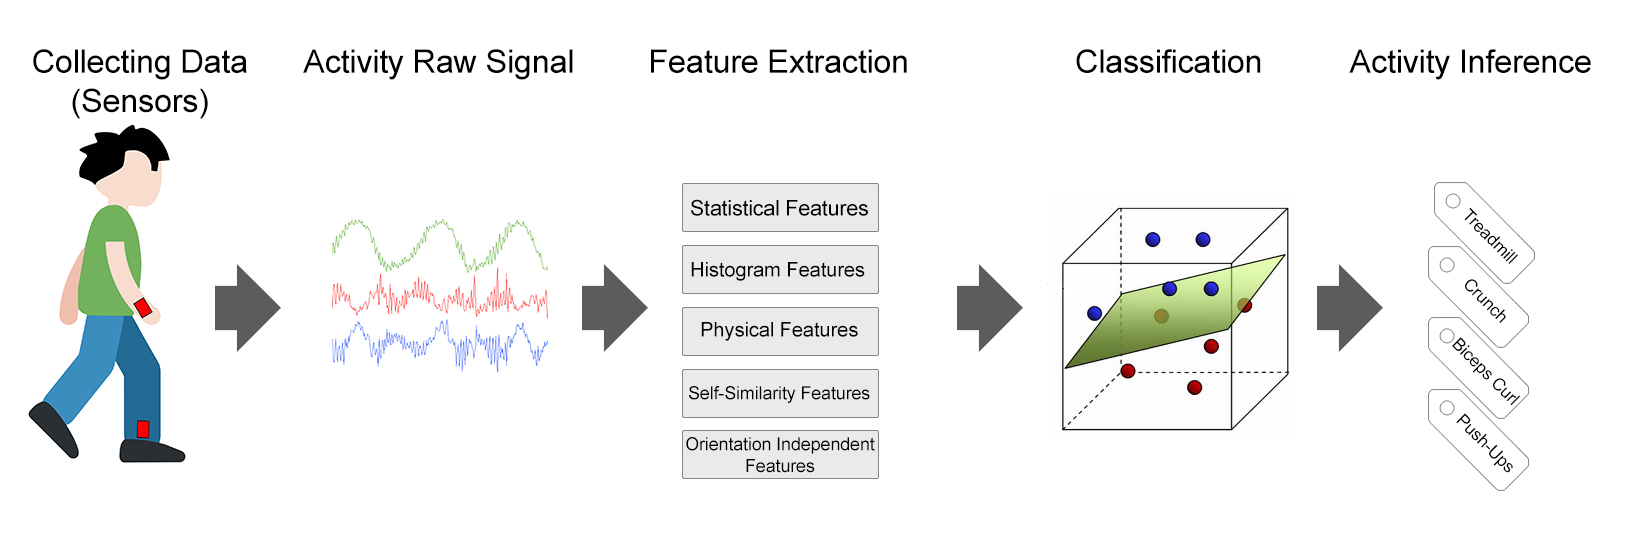
\includegraphics[width=14 cm]{Definitions/images/main_approach.jpg}
	\caption{Typical Work-flow on Human Activity Recognition}
	\label{fig:main_approach}
\end{figure} 
The data collected by sensors as \textit{activity raw data} is the input for Human Activity Recognition (HAR) model\cite{rosati2018comparison}. A HAR model classifies certain activities from input signal which consists of three phases: First, there is a processing operation to \textit{extract features} from raw signal. Then, in \textit{classification }phase there is a classifier to discriminates activities. Finally, in the third phase, there is an \textit{evaluation} method to ensure that the classification provides required performance\cite{kolodziej2019registration}.  Figure \ref{fig:main_approach} shows a start-to-finish pipeline of HAR.\\

To recognize an activity, selecting a proper set of features from raw data plays an important role in the HAR performance \cite{zhang2013human}. Basically, a feature might be acquired from a statistical function (e.g., mean, variance), or a transformation function (e.g., Discrete Wavelet Transform, Fourier Transformation), or a combination - hybrid of them \cite{wang2019survey}. Depends on the function that is in-use, features are coming at different levels of cost and complexity. Additionally, different features are not necessarily informative equally. Therefore, extracting the most valuable features at the expense of minimum cost of computation is the main goal in \textit{feature extraction} phase. Previous works have proposed a wide range of features for HAR models \cite{janidarmian2017comprehensive, wang2019survey}. Although the cost of extracting a feature can be measured by calculating the complexity order of the function, the impact of a feature on the performance of the model is something not achievable theoretically\cite{rosati2018comparison}. Therefore, we need an empirical study on hand-crafted features to assess their impacts on performance.\\
The goal of this paper is to examine the impact of different features on wearable-based HAR. Specifically, we aim at examining five state-of-the-art featuresets (RQ1) and performance of classifiers on each featureset(RQ2) through a start-to-finish pipeline HAR system. Furthermore, we investigate the performance achieved by models under three evaluation methods (RQ3).


Study on validation protocols to choose a reliable method to assess an HAR model \cite{jordao2018human}(in the phase 3)

%(3) impact of quality of dataset on performance since they vary from paper to paper\cite{jordao2018human}.\\
%While the first two issues have impact on performance of a model in general, the third one influences directly on recognition result, independent from how much a model is well designed. Factors like size of dataset, frequency rate of sensors, complexity of target activities, sensor position and how it is attached to the body, and so on. In [], the authors, looking for impact of sensor alignments, in two different trials attached the sensor to the subjects. In first trial, an expert attached the sensor while in the second trial, subjects were asked to attached the sensors by themselves. Results show that the performance has a significant collapse during the second trials.
%
%Regarding the first issue, previous works have employed a wide range of features for HAR models. Dealing with selecting appropriate features (feature extractions/selection) are usually aiming to improve the performance and/or decreasing the computational costs. Previous works have proposed a wide range of features to be extracted as well as feature selection methods to choose the most appropriate featuresets. Some studies also have presented some featuresets that are manually selected based on the context (e.g., type of the activity). In our previous work\cite{Nourani_CoMoRea2019}, we showed that by removing redundant features, we can keep the performance identical while shrink the dataset to 8\% of its initial size. This approach significantly decreases the processing cost and vulnerability of getting overfit. In this study, we will also focus on improving performance by choosing the right featureset rather just decreasing size of dataset in a feature-set.\\
Addition to this, in \cite{rosati2018comparison} which is the most similar previous work to us, the authors also listed two extra issues which less have been considered in previous works:
(1) The processing cost of producing a feature
(2) The complexity of calculation of features makes a model difficult to understand.
we also mention these aspects in this study.

While choosing an appropriate featureset plays an important role to improve the performance of the model, study on validation methods is a critical point since different validation methods show performance differently. For the same reason, using HAR models on new dataset shows a significant decrease in performance. As a consequence of this issue, currently it is impossible to know the state-of-the-art methods in human activity recognition\cite{jordao2018human}. Addition to this, some factors like temporal changes in user body (e.g., tiredness) have impacts on how they perform an identical activity within two different trials. However, it is impossible to evaluate such impacts by traditional validation methods like k-fold cross-validation or Leave-One-Subject-Out (LOSO) cross validation. To address this issue, in this study, we employ Leave-One-Trial-Out (LOTO) cross-validation addition to conventional validation methods.\\

A typical work-flow on human activity recognition is including feature extraction, classification and evaluation (Figure \ref{fig:main_approach}).


The aforementioned discussion motivated our study, where we evaluate a wide range of features by the performance reached by four popular classifiers. The models train and evaluate on our dataset which is one of the biggest dataset on gym exercises, publicly available. To provide a more robust evaluation we validate our models under several cross-validation methods including K-Fold, LOSO, and LOTO.

The aim of this article is to present the following main contributions:
\begin{itemize}
	\item Study and evaluation of the remarkable state-of-the-art featuresets.
	\item Analysis and interpretation of a novel model using Forward Neural Network (FNN) in HAR
	\item Study on validation methods and their vulnerabilities in HAR.
\end{itemize}
%Regarding the target datasets, we chose [] dataset since it provides a wide range of activities (33 activities) and it is big enough.
To the best of our knowledge, there is no dataset that targets different trials of same activity with same subject, publicly available. So, we collected a dataset of 13 subjects and +50 gym activities including different trials for each activity.

The rest of this paper is organized as follows. Section 2 describes the study setup including the approach and the dataset used in this study. Section 3 defines the featuresets and theirs advantages in previous works. Section 4 presents the results of using featuresets on classifiers. Finally, Section 7 summarizes this study and highlight the most important contributions of this paper for future works.
\section{Related Work}




Basically, a HAR system using Inertial Measurement Units (IMUs) is composed of two basic components: (1) a data acquisition unit responsible for capturing human movements, (2) a processing unit responsible for recognizing the certain activities among movements of the subject\cite{rosati2018comparison}. In the first component, the human movements is captured by different motion sensors such as accelerometer, gyroscope, and so on. These sensors can be located in an off-the-shelf device like a smart-phone for general HAR applications or specifically are accompanied by a storage and a processor, formed a System on Chip (SoC) for a certain purpose. The captured movements as raw data transmits to the second component for processing operation.\\
Within the processing unit, there is a pattern recognition (HAR) model that classifies the input signals into certain classes of activities. This HAR model typically consists of three phases. First, there is a pre-processing operation that extracts informative features from raw signal. Second, a classifier is trained over extracted features. Third, an evaluation method to ensure that the classifier provides the required performance\cite{kolodziej2019registration}. In other words, a HAR model should address these three aspects to be able to recognize an activity.


In literature, in order to gain more information from the sensory data, the authors came up with hundreds of hand-crafted features among time domains, frequency domain or a combination of them. While each feature represents the signal in a certain point of view, it does not mean that this feature is informative enough for a model to recognize an activity based on that. One decisive factor to build a new feature is respecting the type of activity. Wang et. al. in \cite{wang2019survey} categorized human activities based on velocity and complexity (number of phases) of an activity into three main groups: (1) The \textbf{basic activities} which happen in comparatively longer duration e.g., walking and running. (2)  The complex activities that are in the form of a sequence of several phases. Each phase might be a complex or basic activity e.g., coffee time, smoking. (3) Transition activities which having a certain but temporal pattern happening between two different postures or two basic activities. e.g., stand-to-sit, push-ups and so on. From this point of view, previous works introduced  different feature sets that each one target a given type of activity. Consequently, targeting more than one type of activity brings more challenges for researcher to create a suitable set of features. Since exercises in gym composed of an orchestration of different type activities (basic, transition, complex), presenting a model to effectively recognize these activities will be more challenging.

Basically, given a stream of sensory data, features are in three main categories.\cite{wang2019survey} 1) Time-domain features, 2) Frequency-domain features, 3) Hybrid features - any combination of statistical functions on signal in frequency-domain and/or time-domain. 

To the best of our knowledge, the statistical functions on time-domain signal provide the most popular features in HAR. Features like mean, median, mean standard deviation, variance, minimum, maximum are the most popular ones. The second group, Frequency-domain features are so helpful for those models that target periodic activities like walking. To achieve a frequency-domain feature, one segment of time signal should be transferred to several components in frequency domain. Each component may/may not have meaning depend on the activity. Frequency bins and auto-correlation coefficient are some example.[available here]

In feature extraction phase, the challenge is to extract the most informative set among a wide range of features\cite{krishnan2009recognition}.  In this regards,


Time-domain features are those features obtained directly from a window of sensor data and are typically statistical measures.  Lots of studies used statistical features in their work because of the reasons mentioned above as well as the low computational cost of them.


%Comparing the two feature subsets, no significant differences were observed for every dynamic activity using SVM and DT, while FNN fed with FeatSet_B was not able to reach acceptable results. \cite{rosati2018comparison}


in \cite{Suto et al., 2017} investigate the efficiency of the popular machine learning strategies based on a right-ankle-mounted accelerometer, and their results suggest that one sensor is not enough for appropriate daily activity recognition due to the similar data generated from one sensor for different activities. Nevertheless, using one sensor can be used as a suitable setup for the basic recognition tasks, such as step counting or sleep quality monitoring. Placing more sensors on multiple body parts is intuitively beneficial for improving the performance and robustness, whereas this can also result in increased complexity in deployment and computation cost. In \cite{Sztyler et al.}, authors developed a position-aware HAR system by placing seven accelerometers in different body positionsl
\section{Data}

The most crucial requirement to start an activity recognition process is having the real-world data of human activities. Although there are couple of datasets publicly available for HAR\cite{wang2019survey}, to the best of our knowledge, non of them provide the data of different sessions (neither at same day or different days) of same subject. In addition, they mostly focused on daily routine activities rather transition activities (e.g., gym exercises) which are repetitive and more complicated in terms of pattern recognition\cite{wang2019survey}. Therefore, in this study we collect a dataset providing the following features:
\begin{itemize}[leftmargin=*,labelsep=5.8mm]
	\item Specifically targeted on regular gym activities (including 55 exercises)
	\item The data tracks activities of a set of subjects over two to six weeks
	\item Data is recorded by four sensors (two wrists and two foots)
	\item Subjects performed the practices only based on their own experiences (there is no instruction) 
\end{itemize}
In this regard, the first step is to determine the sensor type and how to deploy a system to collect the data. In this work, we have employed a SoC device which called \textit{Neblina}.
\subsubsection{Neblina}
Neblina is a miniature-sized box containing three tri-axial motion sensors (accelerometer, gyroscope, magnetometer) along with a processor, a flash memory, battery, and a bluetooth port. Using blue-tooth port, it can transmit the result to a host (e.g., cellphone or desktop computer).  In fact, Neblina is equipped with all requirements for a real-time HAR system. Comparing with a smartphone, Neblina is much smaller (Figure \ref{neblina_setup}) that lets us to attach it to different part of the subject's body without making any interrupt in his/her actions\cite{de2018comparative}. Having access directly to different resources like sensors or memory without OS interferences is another advantage of using Neblina that let us improve the efficiency of the model.
\begin{figure}[H]
	\centering
	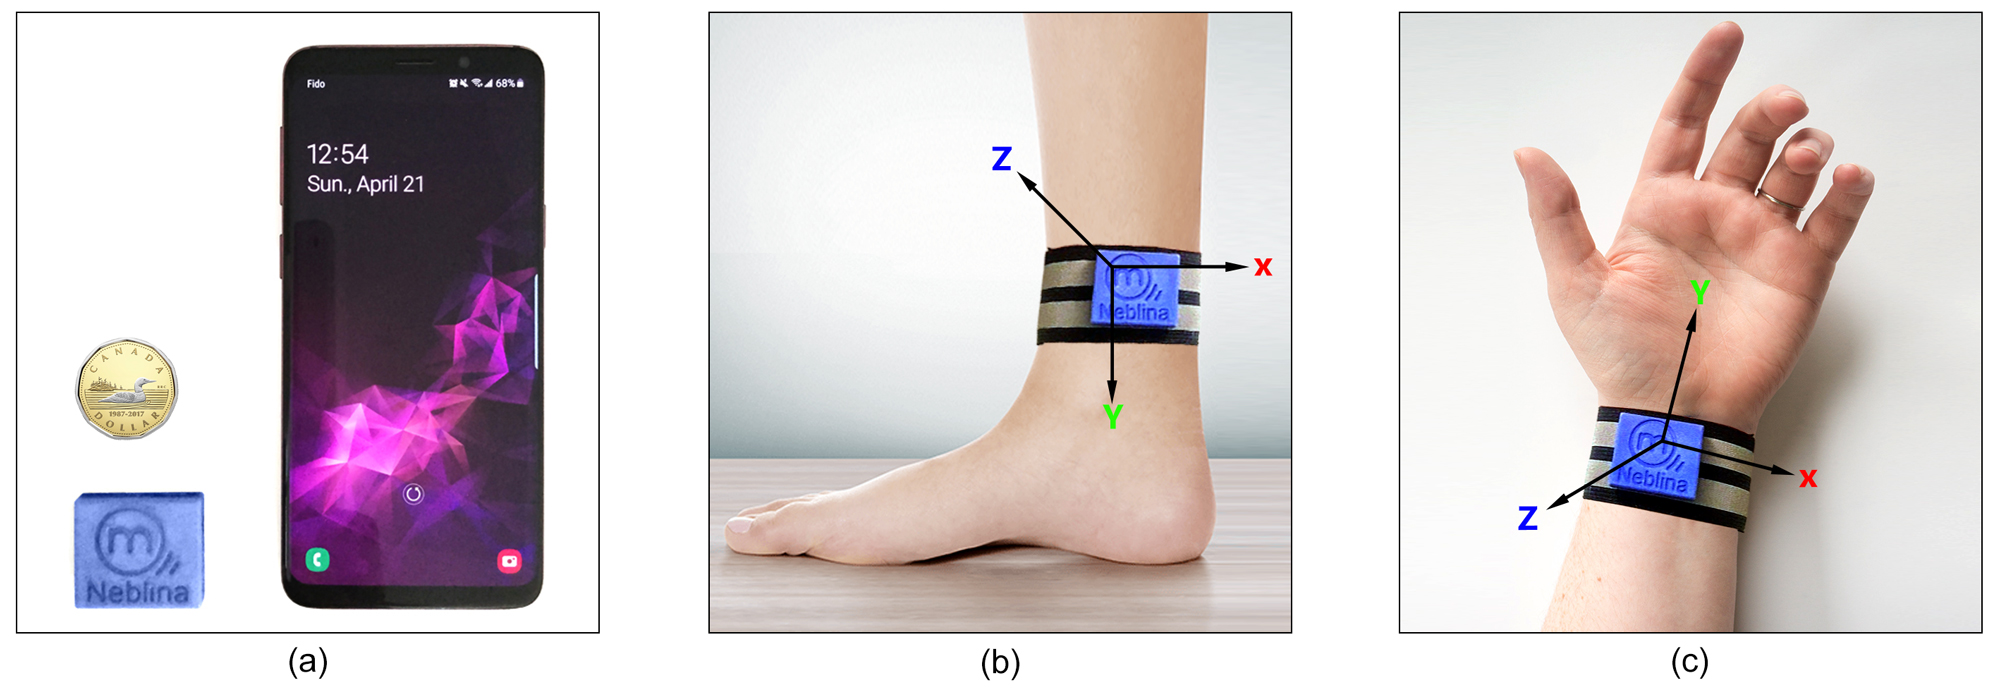
\includegraphics[width=10 cm]{Definitions/images/neblina_setup.jpg}
	\caption{Neblina setup. (a) Compares dimensions of Neblina with a 1 dollar coin and a cellphone (Sumsung Galaxy s9). (b) How Neblina located on foot using a strap. (c) How Neblina located on wrist using a strap.}
	\label{neblina_setup}
\end{figure} 
\subsubsection{Sensors} 
Depending on how much an activity is complicated (e.g., how many parts of body are involved or how many stages it contains), a researcher may need to attach one or more sensors on different positions of the human body. However, using more sensors affects usability negatively. From the literature, using sensor on wrist for most of upper body activities and using a sensor on foot for lower-body activity are more effective than other locations including chest, waist, thigh and so on. In this study, to cover activities both on lower-body and upper-body, two sensors were attached to right wrist and right foot (Figure \ref{neblina_setup} (b) and (c)). Although the device provides the magnetometer signals, we limited our process on using the accelerometer and gyroscope signals only. It is because the magnetometer signal can be affected by getting close to iron equipments in the gym. The frequency rate is fixed on 50Hz. It is worth to mention that the frequency rate more than 50Hz is not necessary because according to the Nyquist theorem, this rate is enough to record a repetitive activity with 25 cycle per second which is so much faster than the iterations of normal workouts in the gym (one iteration per 1-5 seconds).\\
\subsection{Subjects}
We asked 15 members of a gym (4 female), ages 21-35, to participate in this study. Participants varied in level of expertise (from 1 month to 6 consecutive years of experience). For more realistic scenarios, we did not constrain participants to certain set of exercises, instead we asked them to follow up their own exercise plan. Comparing with previous works' dataset, considering this level of freedom for subjects returns following advantages: (1) Since each session is about 1 to 2 hours, we can observe the impact of fatigue on performing an activity. (2) The unknown period or null-class activities are not artificially performed, since subjects were free to do whatever they normally do in gym (3) impact of background experience can be measured. It is because the gym programs are cyclic over week or month. By repeating an activity over cycles, Subjects will be more consistent over different sets ( a consecutive sequence of doing one activity). (4) there is no instruction of how doing exercises for subjects. Although this can let subjects to perform an activity in non-identical way, it is considered as an advantage for our study since it replicates the real-world condition. In \cite{morris2014recofit}, the authors showed that by changing the environment from space-constrained laboratory to a real gym the segmentation performance for recognizing gym exercises has dropped by 50\%. Therefore, another advantage of keeping the experiment under real-world condition is the performance of the model is more reliable.\\
\subsection{Activities}
Our dataset ended up with 55 common exercises in gym. During electing participants, we picked mostly those persons who do more common exercises involved in either upper body or lower body. Thus, activities like Wall ball, jumping jacks and so on or advanced exercise in body-building are not in our dataset. In \cite{soro2019recognition} (the second dataset in this work), authors have targeted CrossFit activities which are involved in upper and lower body together. They have shown that only one sensor on wrist is enough to recognize such activities. Therefore, in this study we focused on those exercises in which either lower or upper body keeps stable during the activity. Thereby, existing the second sensor is necessary for recognizing the activity. As listed in Table \ref{activity_list}, only two activities are involved in both upper and lower body. Running on treadmill (A1) make lower body involved. While In previous works this activity was recognized by sensor on wrist. Since a user can put her/his hands on device handler, using sensor on wrist is not effective always. \\
\hosein{Recognition accuracy is assessed in the context of a circuit, and inevitably the choice of circuit affects accuracy. A larger number of activities or high similarity among activities will reduce accuracy. Comprehensive analysis of all possible circuits is prohibitive, so we present results from the two circuits used in our study, along with leave-one-out cross-validation results from our training data for two reasonable circuits of different sizes, to demonstrate the effect of circuit size on accuracy.}
\begin{table}[H]
	\caption{List of exercises along with target body part involved in each exercise.}
	\centering
	%% \tablesize{} %% You can specify the fontsize here, e.g., \tablesize{\footnotesize}. If commented out \small will be used.
	\begin{tabular}{ccc}
		\toprule
		\textbf{Exercise}	& \textbf{Body Involved}	& \textbf{Code}\\
		\midrule
		Lat Pull Down		& upper 		& A1\\
		Bench Press		& upper 			& A2\\
		Biceps curl		& upper			& A3\\
		Push-ups & upper			& A4\\
		Treadmill		& lower 			& A5\\
		Ab crunch machine		& lower \& upper & A6\\
		Reverse Crunch & lower			& A7 \\
		Russian Twist & lower			& A8 \\
		\bottomrule
	\end{tabular}
\label{activity_list}
\end{table}
\subsection{Data points}
To generate the data points, previous works have employed different strategies. One well-known method for time-series signals is sliding-windows. As long as an activity is squashed in a range of samples during time, a model can see a stream of recorded data through a window with limited length of seconds (e.g., in this study it is 5 seconds time window). This window slides through the stream with a certain step size called shifting size. As long as the shifting size smaller than widow size, the sliding window is called overlapping and non-overlapping if they are equal. Previous works have shown that the different lengths of window size and shifting size influence the performance of the model and the computational cost. Because the activities in this study are gym exercise which the do not take longer than 5 seconds, intuitively, we choose 5 seconds for window size. It is a safe window size to ensure that at least one cycle of the activity can be completely seen in a window frame. we defined 200 milliseconds for shifting step which keeps the model more sensitive against changes in signal at the expense of more computational cost. Having such small shifting step does make sense since in real-world applications it decreases the latency of the application on predicting the activity type. Addition to the time period, the window length can be defined by the sampling rate of sensor. In this work, the sample rate is 50Hz. So, each window contains 250 (5 * 50) samples.

\subsection{Dataset}
To label the data we employed a process including three phases: (1) Before beginning of each session, each subject was asked to fill a form about list of activities, number of sets, and the weights if applicable. (2) During the session, a supervisor manually records type of exercise, the moment of start and stop, and number of repetitions. (3) After finishing the session, in order to have our desired accuracy in labelling, we visually trace the signals of accelerometer and gyroscope to refine the regains assigned to each exercise.
Table \ref{dataset_statistics} shows the statistics of the dataset. Since subjects may participate in more than one session, next column after subjects, shows the total number of sessions for each activity.  , in the initial dataset, the number of subjects who are involved in all exercises is not equally distributed. Although  Thus, we defined four datasets corresponding with our four experiments including K-fold evaluation, Leave-One-Set-Out evaluation, Leave-One-Session-Out evaluation, and Leave-One-Subject-Out evaluation.
\begin{table}[H]
	\caption{Statistics of the dataset divided by type of exercise along with the experiments that involve them in.}
	\centering
	%% \tablesize{} %% You can specify the fontsize here, e.g., \tablesize{\footnotesize}. If commented out \small will be used.
	\begin{tabular}{ccccc}
		\toprule
		\textbf{Exercise} & \textbf{Subjects} & \textbf{Sessions}	 & \textbf{Reps} & \textbf{Samples}  \\
		\midrule		
		Lat Pull Down& 6& 22& 218& 14700\\
		Bench Press	& 6& 26& 273& 23230\\
		Biceps curl	& 4& 13& 115& 16095\\
		Push-ups & 5& 16& 181& 9200\\
		Treadmill& 4& 5& +1200 & 68780\\
		Ab crunch machine& 4& 12& 108 & 10580\\
		Crunch Twist &  3& 12& 98& 8760Yes\\
		Russian Twist & 3& 8& 67& 8520\\
		\bottomrule
	\end{tabular}
	\label{dataset_statistics}
\end{table}


\section{Method}
As mentioned above, in addition to data collection, a HAR process encompasses, feature extraction and activity recognition (i.e., classification). In addition, we typically employ a number of validation techniques to examine the effectiveness of the validation. In this section, we describe the aforementioned part of a HAR process.

\subsection{Feature Extraction}

To perform our study, we extracted five sets of features from our dataset. To create the features, we applied a comprehensive range of functions, detailed in previous work, directly on tri-axial input signals of acceleration and gyroscope from sensors on wrist and foot (12 input signals) \cite{morris2014recofit, yurtman2017activity, zhang2011feature, Sarbishei2019platform} \todo{add cites}. Table \ref{features_table} shows functions along with a description/intuition about each feature. Based on the main advantage of each group of features, we wrap them into  feature sets. In other words, each set is uniquely representative of a certain aspect of the signal stream we gathered from the sensors. 

\textbf{Preprocessing.}  \todo{add reason...} \hosein{To ensure that the data from different sensors are on the same scales}, we performed a scale normalization to extracted all features, which scales the input signals into a range between 0 and 1. In certain cases, we performed specific preprocessing operations, which are only specific for a certain feature set (which we explain within). Next, we describe the five feature sets.

\subsubsection{Set\_A: Statistical Features (ST\_Set)}
Statistical features have been intensively investigated in different applications and proved to be effective and useful for HAR~\cite{rosati2018comparison}. These features are based on a comprehensive and intuitive understanding of how a given activity produces a set of discriminative features from measured sensor signals. We created a set of 264 features obtained by applying 11 statistical functions on 24 input signals, including (x/y/z axes of accelerometer and gyroscope, along with the cumulative sums of each axis). Functions are used in the statistical feature set are indicated by the code S1-S11 in Table~\ref{features_table}. 

\begin{table}[H]
	\caption{Statical Functions along with the definitions and abbreviations }
	\centering
	%% \tablesize{} %% You can specify the fontsize here, e.g., \tablesize{\footnotesize}. If commented out \small will be used.
	\begin{tabular}{p{0.9cm}p{5cm}p{7cm}p{1.3cm}}
		\toprule
		\textbf{Code} & \textbf{Function} & \textbf{Description/Intuition} & \textbf{{\scriptsize abbreviation}} \\
		\midrule
		{\footnotesize S1}&Minimum & {\scriptsize The value of the least sample}& MIN\\
		S2&Maximum & {\scriptsize The value of the greatest sample}& MAX\\
		{\footnotesize S3, SS8}&Mean&  {\scriptsize The average of all samples}& MEA\\
		{\footnotesize S4}&Median&  {\scriptsize The middle value of samples}& MEA\\
		{\footnotesize S5}&{\footnotesize Mean Absolute Deviation}& {\scriptsize The average distance between each sample and the mean of the stream}& MAD\\
		{\footnotesize S6}&{\footnotesize Median Absolute Deviation}& {\scriptsize The average distance between each sample and the median of the stream}& MAA\\
		{\footnotesize S7}&Inner Quartile Range  & {\scriptsize The amount of spread in the middle part \%50 of the stream}& IQR\\
		{\footnotesize S8}&Mean Crossing Rate& {\scriptsize The rate of passing the mean along the stream}& MCR\\
		{\footnotesize S9, SS9}&Standard Deviation& {\scriptsize how far the samples are from the mean}& SD\\
		{\footnotesize S10, SS10}&Variance& {\scriptsize the average degree of distance between samples and mean}& VAR\\
		{\footnotesize S11, SS11}&Root Mean Square& {\scriptsize The square root of the arithmetic mean of the squares of samples}& RMS\\
		{\footnotesize HB}& Histogram Bin&{\scriptsize a 20 bins distribution of data } & Hbin (1-20) \\
		{\footnotesize SS1}&Number of autocorrelation peaks& {\scriptsize \hosein{???}The greater number of peaks refers to non-periodic activity and vice versa. }& NAcP\\
		{\footnotesize SS2}&Prominent autocorrelation peaks&{\scriptsize NAcP with an extra condition that the peaks should be greater than neighbours with at least a certain distance} & NAcPP \\
		{\footnotesize SS3}&Weak autocorrelation peaks&{\scriptsize NAcP with an extra condition that the distance between the peaks and neighbours should be less than a certain distance} & NAcWP \\
		{\footnotesize SS4}&Maximum autocorrelation value&{\scriptsize Value of the greatest peak (except for the initial peak at zero lag)} & MAXAc \\
		{\footnotesize SS5}&Height of the first autocorrelation peak (after zero-crossing)&{\scriptsize less height refers to more fluctuations within the stream  } & FAcP \\
		{\footnotesize SS6}&Power bins (10 bins)&{\scriptsize A 10 bins distribution of amplitudes of frequencies from 0.2-25Hz    } & Pbin(1-10) \\
		{\footnotesize SS7}&Integrated RMS&{\scriptsize The root-mean-square amplitude of the signal after cumulative summation } & IRMS \\
		Ph1&Movement Intensity&{\scriptsize the Euclidean norm of the total acceleration vector after removing the static gravitational acceleration } & MI\\
		Ph2&Normalized Signal Magnitude Area&{\scriptsize the acceleration magnitude summed over three axes within each window normalized by the window length } & SMA \\
		Ph3&Eigenvalues of Dominant Directions&{\scriptsize The eigenvectors of the covariance matrix of the acceleration data correspond to the dominant directions along which intensive human motion occurs.} & \\
		Ph4&Correlation between Acceleration along Gravity and Heading Directions&{\scriptsize It shows the human movement is either vertically or horizontally. } &CAGH \\
		Ph5&Averaged Velocity along Heading Direction&{\scriptsize The Euclidean norm of the averaged velocities along y and z axes over the window.} &AVH \\
		Ph6&Averaged Velocity along Gravity Direction&{\scriptsize averaging the instantaneous velocity along the gravity direction at each time t over the window } & AVG \\
		Ph7&Averaged Rotation Angles related to Gravity Direction&{\scriptsize The cumulative rotation angles around gravity direction} & ARATG \\
		Ph8&Dominant Frequency&{\scriptsize The frequency corresponding to the maximum of the squared discrete FFT component magnitudes of the signal from each sensor axis} & DF \\
		Ph9&Energy&{\scriptsize The sum of the squared discrete FFT component magnitudes of the signal from each sensor axis} & ENERGY \\
		Ph10&Averaged Acceleration Energy&{\scriptsize The mean value of the energy over three acceleration axes} & AAE \\
		Ph11&Averaged Rotation Energy&{\scriptsize The mean value of the energy over three gyroscope axes. } & ARE \\
		OI1&Orientation Independent&{\scriptsize result of applying PCA on Single Value Decomposition  of x/y/x values of the stream } & PCASVD(1-30) \\
		%		&&{\scriptsize } & \\
		%		&&{\scriptsize } & \\
		%		&&{\scriptsize } & \\
		\bottomrule
	\end{tabular}
	\label{features_table}
\end{table}


\subsubsection{Set\_B: Histogram bins Features (HB\_Set)}
The second set of features are based on histogram representation of time series signal. Mathematically speaking, histogram representation of a signal is the probability distribution of signal over a period of time (often referred to as window size)~\cite{zardoshti1995emg}. In HAR, considering the fact that each activity contains a set of small movements (as small as one sample) with certain acceleration and rotation, histogram bins indicate the difference between activities by showing the different distributions of those small movements. Shirahama et. al.~\cite{shirahama2016codebook} used a histogram-based feature set for HAR. Comparing with statistical features, histogram bins have a significantly lower cost in terms of required processing time and memory usage~\cite{Sarbishei2019platform}. However, they are sensitive against the resolution/granularity of bins (count and width of bins). Following prior work~\cite{xi2017evaluation}, in this work, we consider 21 bins for values between 0 through 1 of a signal. Histogram bins are indicated with the code HB in Table~\ref{features_table}.


\subsubsection{Set\_C: Self-Similar Features (SS\_Set)}
%As formerly mentioned, having enough number of bins, histogram can represent the distribution of data. However, it can not show the periodic attributes of a signal over time. 
Considering that an exercise activity is inherently more repetitive rather than a non-exercise activity, having a featureset that can capture the repetitive behaviour of signal is helpful. Morris et. al. presented a featureset designed based on the idea of extracting repetitions forms of signal \cite{morris2014recofit}. These features can be extracted by calculating the convolution of a signal with a shifted version of itself (autocorrelation) or by extracting the components of the signal in the frequency domain. We extracted a number of self-similar features from our data, as shown in~Table~\ref{features_table}, features with code SS1-SS11 \emad{In the table, the SS features do not make sense.}\hosein{updated their descriptions. check it please.}. SS6 composed of 10 power bins \emad{what are power bins?} \hosein{for example after applying Fourier transformation on 250 samples(5s), we have 125 frequencies (Nyquist). these frequencies start from 1/5Hz through 25Hz. In this case, I split 125 frequencies into 10 groups based on certain frequency band. Then, for each group, calculated the magnitude of each frequency and summed them together. it is roughly similar to histogram bins but in frequency domain. }.
\hosein{Resembling the study of Morris et. al \cite{morris2014recofit}, as the preprocessing operation, we transformed 3 input signals from each sensor (x/y/z inputs) to 4 processed signal describing as follows: 1) The magnitude of a/y/z axes, 2) The first principal component of all axes. 3) The first principal component of y and z axes. 4) The scaled normalized of y axis. It is important to mention that in our experiments, the y axis of sensor is along the user's arm. To build the featureset, we applied 20 functions on 16 processed signals (two accelerometers and two gyroscopes). These functions indicated by "SS" prefix are described in \ref{features_table}. Therefore, this featureset contains 320 features. }
In total, we applied 20 functions on the raw values of the y-axes \emad{y-axes? why only y-axes?} of sensors along with three processed signals as follows: 1) the magnitude of all axes of each sensor (two inputs); 2) the first principal component of all axes of each sensor (two inputs); and 3) the first principal component of y and z axes of each sensors (two inputs). Therefore, in total this featureset has 320 ( 2 * 8 * 20) \emad{what are the 2, 8 and 20 here?} features. It is important to mention that in our experiments, the y vector is along the user's arm. 

\subsubsection{Set\_D: Physical Features (PH\_Set)}
One intuitive idea to design a set of features from sensory data is to take the principles of human movements into consideration. In 2011, Zhang et. al. ~\cite{zhang2011feature} introduced a set of features based on physical parameters of human motion. To have a strong physical meaning of motion data (e.g., moving forward, backward), they assumed that the sensor position and direction are known during the experiment. In other words, this types of features is derived based on the physical interpretations of human motion, called physical features. Comparing with other featuresets, these features are made up of a fusion of multiple sensor inputs rather than just one inputs sensor. In our paper, this featureset contains 11 features, labeled with the code Ph1-Ph11 in Table~\ref{features_table}. As a part of our pre-processing operation, we remove gravity from acceleration using gyroscope data by applying the method described in~\cite{Accelero5:online}.

\subsubsection{Set\_E: Orientation Independent Features (OI\_Set)}
In contrast to physical features, which depend on the position and orientation of sensors, Yurtman et. al~\cite{yurtman2017activity} proposed features that do not rely on variation of sensor orientation. In fact, in their model, they introduced an Orientation-invariant transformations (OITs). They compared their model with the ordinary model - pre-defined sensor orientation, on five different datasets. Although their featureset did not have a significant impact on performance, it brought an extra added value to the model that lets it to be more robust against orientation. The OIT that they have introduced in their work is inspired by the idea of \textit{single value decomposition}\cite{moon2000mathematical}. Therefore, to create this featureset, first, we project every data point from original x/y/z space to a new space with same number of dimensions but at the farthest distance between data points. The intuition here is that the direction of the axes are defined by value of the data points not by x, y or z direction. Next, we apply PCA on the transformed data and take the first 30 most informative features \cite{janidarmian2017comprehensive} \todo{can we add a cite here?}. In Table~\ref{features_table}, these type of features  are indicated by "OI" prefix.

\subsection{Activity Recognition}
To perform the HAR, we employed a number of classification techniques. In this subsection, we detail the classification techniques used.

\subsubsection{Support Vector Machine}
A multiclass Support Vector Machine (SVM) has been used to discriminate among the activities. Assuming each data point is a co-ordinate (support vector) of feature space, the Support Vector Machine (SVM) is an algorithm to find an optimum hyperplane between support vectors between two classes. To create a more robust classification, SVM maximizes the distance between the hyperplane and the closest support vectors of each class (margin) \cite{zhang2012physical}. We chose to use SVM since it has been employed extensively in previous studies in HAR. Moreover, Morris et. al.~\cite{morris2014recofit,rosati2018comparison} showed that SVM provides high accuracy in HAR.


% More Details: This happens at the expense of increasing the tolerance(mis-classification) of the model (loss function). In a situation that finding a hyperplane between two classes is impossible, the SVM project the feature space to another space having more number of dimensions. This is the responsibility of a function called Kernel function.

\subsubsection{Decision Tree}

We also use a decision tree classifier since it is one of the most commonly used classifiers in HAR \cite{mortazavi2014determining, baldominos2019comparison} and provides explainability for its classification. \hosein{Baldominos et. al. \cite{baldominos2019comparison} achieved best accuracy among different classifiers using DT} Decision trees predict the type of an activity using the average class probabilities at leaf nodes and the highest average probability is chosen as the class label (activity type). There are different techniques to split nodes, however we used the Gini index error metric, which is generally designed to evaluate inequality. We chose to use the Gini index metric since ...\todo{add reasons.} \hosein{since authors in \cite{rosati2018comparison, masum2018human}used it; it is very simple to implement and, it is the default splitting method for decision tree in R (rpart library) }

\hosein{Explanation: Considering we split data points based on values of a feature into several chunks, basically, Gini function returns how "pure" a chunk is. The "Purity" means how much of data in each branch belongs to a certain activity. Greater proportion of an activity in a chunk results smaller value of Gini coefficient for that feature. features with lower Gini index will be located on upper level of tree. splitting continues as long as new chunks have smaller Gini index. }


\subsubsection{K-nearest neighbour}
Another widely used classifier in HAR is the KNN algorithm \cite{wang2019survey,shakya2018comparative}, which is based on the calculation of the distance (in our study the Euclidean distance) between the data point required to be classified and labelled data points in training set.  Firstly, the training sets are sorted in descending order according to their distance from the new element. Then, the most frequent class of the first K elements (called neighbours) is associated to the new element. The majority of neighbours determine the class for a new data point. Prior work showed that by increasing the number of neighbours, they reached a better performance on HAR model. In this study we used k = 64~\cite{kose2012online}.


\subsubsection{Forward Neural Network}
\emad{we should add a sentence as to why we use FNN. For example...}
\hosein{With proper feature design, convention machine learning models (e.g., SVM, KNN) can achieve a good performance in activity recognition. However we can improve it by using Deep Neural Network, which underlies the complementary information learned within the layers \cite{chen2018distilling}.}
Recently, a number of studies have shown that Feedforward Neural Networks achieve high performance in HAR\cite{chen2018distilling, zhu2009human}. A FNN is made up of a set of neurons, connected by weighted arcs, that process the input
information:
\begin{equation}\label{fnn_formula}
 y = f(\sum_{i}^{}w_{i}.x_{i})
\end{equation}
where y is the output of the neuron, $ w_{i} $ are weights of the incoming connections, xi are inputs to the neuron, and $f$ is called transfer function and should be selected according to the classification problem \cite{zhang1999geometrical}. Neurons in a FNN are organized in layers: in the input layer, one neuron for each input variable is required; the number of neurons in the output layer is decided according to the number of classes to be recognized and the selected transfer function; between input and output layers a certain number of hidden layers can be inserted, whose dimensions are usually decided testing different configurations ~\cite{baldominos2019comparison}. 
In the FNN model we used the multi-layers perceptron (MLP), commonly used as a universal function approximator. The first layer of the network (input layer) receives a vector of feature values of a data point. The secondary layers well known as hidden layers are responsible for summation operation of inputs and non-linearity behaviour of network. We considered 3 hidden layers including two dense layers and one dropout layer for out FNN. The activation functions for the first and third layer is "ReLu" \cite{nair2010rectified} with total 1000 and 400 units respectively. The dropout rate in second layer is 60\%. The output layer contains 9 units corresponding with total 8 activities plus 1 non-activity class. Same as similar study in \cite{baldominos2019comparison}, we used Adam optimizer setting a learning rate of 0.0001 and decay = 1e-10. In total, we trained the model by 100 epochs.


\subsection{Validation Technique}
To evaluate the performance of the model, we need to split data into training and testing sets. For this purpose, in the context of HAR, there are traditional techniques such as k-fold cross-validation, leave-one-subject-out~\cite{jordao2018human}, as well as, the relatively less common techniques like hold-out and leave-one-trial-out~\cite{sena2018multiscale}. In this study, we chose three validation methods that are commonly used in the evaluation of HAR models \cite{wang2019survey}. 
%The other methods like leave-one-sample-out or holdout can be considered as different forms of these three methods.

\subsubsection{K-fold Cross validation}
The most typical approach to evaluate the performance of HAR model is k-fold-cross validation. The idea is to use resampling procedure in a way that all the samples be used once during the testing period, mostly in the case of having limited dataset. The so called parameter k refers to the number of groups that the given dataset is to be split into. Each time one group becomes the test set and remaining $k-1$ groups become training set. During k turns, we evaluate the model k times on different test set and train set. Finally, the performance is summarized by averaging the performance of all k turns. In this work, we apply k-fold cross validation on all the models.

\subsubsection{Leave-One-Subject-Out Cross validation}
Leave-One-Subject-Out (LOSO) validation is a special case of cross-validation, where a subject can be seen as a fold, hence, the number of subjects determine the number of folds. Furthermore, the LOSO validation technique reflects a realistic scenario, where a model is trained in an offline way, using the samples of some subjects, and is tested with samples of unseen subjects. It is important to note that using LOSO may present high variance in performance from one subject to another, since the same activity can be performed in different ways by the subjects. 

\subsubsection{Leave-One-Trial-Out Cross validation}
The Leave-One-Trial-Out (LOTO) cross validation is similar to LOSO, however, instead of considering the subjects as folds, each trial (session) of doing the activity is considered as a fold \emad{is it folds across subjects or within the same subject?}. In other words, the recorded data from each session has an identifier to be distinguished from other sessions. So, during the evaluation, the dataset is split into sessions instead of subjects. sessions can be for same subject or different subjects. In our dataset we also put an extra column showing the session $id$, which is unique among all sessions of a given subject. The main advantage of using this process comparing with the previous one is that it needs a smaller number of subjects since each subject can have several sessions. And same as to other validation techniques, there is no overlap between train set and test set.


\subsection{Performance Measures}

Some of the most commonly used performance measures to determine the performance of HAR models used in prior work are: accuracy\cite{brownlee2018gentle,zhang2011feature,mehrang2017human} and F-measure\cite{rosati2018comparison,Nourani_CoMoRea2019}. While accuracy is a straight forward measure to show the performance of the model, F1 is also a suitable measure since it relies on both the precision and recall; knowing, it is less affected by unbalanced classes. Specifically, measurement units in this study determined as follows:

\begin{itemize}

\item \textbf{True Positive (FP):} These are cases in which we predict an activity, and user was doing that activity.\\

\item \textbf{True Negative (TN):} Is where we predict a non-activity period, and user was not doing a certain activity.\\

\item \textbf{False Positive (FP):} Is where we predict a certain activity for a segment of data, however, user is either doing another specific activity or generally doing something else (out of activity given list)\\

\item \textbf{False Negative (FN):} Is where we predict either a not-activity period or a certain activity, but, it is not the activity that user is really doing that.\\

\end{itemize}

The most popular metrics are the following:\\

\begin{itemize}

\item \noindent \textbf{Accuracy} measures how often the classifier is correct. Specifically, it is equal to (TN + TP) / total.\\

\item \noindent \textbf{Miss-classification} measure how often the classifier is incorrect. Specifically, it is equal to (1 - Accuracy).

\item \noindent \textbf{Precision} measures when the classifier detects an activity, how often it is  correct. Specifically, it is equal to TP / (TP + FP). \\

\item \noindent \textbf{Recall} measures when user is doing a certain activity, how often the classifier can detect it correctly. Specifically, it is equal to TP / (TP + FN). This term is also known as \textit{Sensitivity} or \textit{True Positive Rate}.\\

\item \noindent \textbf{F-Score} measures a weighted average of both Recall and Precision. Specifically, it is equal to (2 x Precision x Recall ) / (Precision + Recall). \\

\item \noindent \textbf{Null Error Rate:} measures how often it is incorrect if we constantly return the major class in dataset as response of the classifier. To the best of our knowledge, in most HAR datasets, the major class is non-activity class.\\

\end{itemize}




\section{Results}
Our study aims to perform a systematic examination of HAR. Therefore, we answer three RQs in our study that focus on the featuresets used in HAR (\textbf{RQ1}), the classifiers use in HAR (\textbf{RQ2}) and the impact of different evaluation methods on HAR's performance (\textbf{RQ3}).

\subsubsection{RQ1: Which featureset provides the best performance in HAR?}

As motivated earlier, choosing an appropriate featureset significantly impacts performance. Many different featuresets have been presented in previous work, with varying levels of performance. Hence, we would like to investigate the impact of each featureset on performance, when all of the conditions (i.e., data, classifiers, etc.) are the same. To increase the generality of answer we train four classifiers including FNN, KNN, SVM, and DT on all five featuresets (20 model in total). We used 10-fold cross validation to measure the performance. A total of 150,000 data points were included in the validation set. 

Table \ref{accuracy_classifier_featureset} shows the accuracy results for each featureset (columns 2-6) for the various classifiers (rows 2-5). We highlight the best performance for each featureset in the Table. It can be seen that the best performing featuresets are \textit{statistical featureset} (ST\_Set) and \textit{Histogram bins} (HB\_Set), achieving an accuracy of approximately 95\%. The remaining featuresets that perform well are the \textit{self-similar featureset} achieving a maximum accuracy of 89.18\%, the \textit{physical featureset} achieving a maximum accuracy of 85.34\% and \textit{Orientation independent featureset} achieving a maximum accuracy of 78.47\%.

It is worth mentioning here that when it comes to the complexity of computing the different features, histogram bins are the least complex to calcualte. Hence, given that they perform so well, they make an ideal candidate featureset, although there are for sure cases where this is not case. At the same time, we do expect that orientation indepedent features to not perform as highly, however, they do allow for flexibility in the way that sensors are placed on a subject.

%classifiers have almost similar behaviour over different featuresets. Almost all classifiers on \textit{statistical featureset} and \textit{Histogram bins} deliver their higher performance which means these two featuresets bring the most informative features rather others. While almost in all featuresets, models are exceeding 80\% accuracy, the orientation invariant features provides insufficient information for successfully tackling activity recognition, since the accuracy never exceeds 77\%. \textbf{Interestingly, the Histogram Features with having the least complexity in computation gained the best performance among other featuresets at 95.89\% when using FNN and 93.30\% on average among all classifier.} In fact, accuracy achieved by the top-performing models (FNN and SVM) are significantly better when they use histogram features. This might happen due to choosing an appropriate bin width based on length of activity and windows size.\\
%We naturally expect the accuracy achieved with the Orientation Invariant featureset to be lower compared to the other featureset since other featuresets (especially physical features) know about the directions of moving and gravity. However, the goal in creating this featureset was to provide the user the flexibility to place the sensor units at any orientation while this ability is not available on other featuresets. 

\begin{table}[H]
	\caption{Accuracy for each classifier and for all each feature-set using 10-fold cross validation \emad{we should only highlight the best performing featureset,i.e., one per column.}\hosein{done}}
	\centering
	\begin{tabular}{p{2cm}p{1.7cm}p{1.7cm}p{1.7cm}p{1.7cm}p{1.7cm}p{1.7cm}}
		\toprule
		\textbf{Classifier} & \textbf{ST\_Set} & \textbf{HB\_Set} & \textbf{SS\_Set} & \textbf{PH\_Set} & \textbf{OI\_Set} & Average \\
		\midrule
		SVM &  94.98\% & 94.55\% &\cellcolor{gray!35}{89.18\%} &84.15\% & \cellcolor{gray!35}{78.47\%} &87.82\%\\
		KNN & 91.50\% & 92.05\% & 85.61\% &81.93\% & 76,41\%& 85.50\% \\
		FNN & \cellcolor{gray!35}{95.31}\% & \cellcolor{gray!35}{95.89\%} &  87.93\% &\cellcolor{gray!35}{85.34\%} & 77.59\% & \cellcolor{gray!35}{89.04}\%\\
		DT & 88.64\% & 89.18\% &  82.94\% &79.37\% & 74.02\% &82.83\%\\
		\bottomrule
		\textbf{Median} & 92.36\% &  92.92\% &86.41\% & 82.70\% & 77.12\%&86.30\%\\
		\midrule
		\textbf{Average} & 92.74\% &  \cellcolor{gray!35}{93.30\%}  & 86.77\% &83.04\% & 77.44\% &86.66\%\\
		\bottomrule
	\end{tabular}
	\label{accuracy_classifier_featureset}
\end{table}
%\begin{table}[H]
%\caption{F1 for each classifier and for all each feature-set using 10-fold cross validation }
%\centering
%%% \tablesize{} %% You can specify the fontsize here, e.g., \tablesize{\footnotesize}. If commented out \small will be used.
%%a = statistical - b=histogram - c=self-similar d=physical feature e=orientation independent
%\begin{tabular}{p{3cm}p{2cm}p{2cm}p{2cm}p{2cm}p{2cm}}
%	\toprule
%	\textbf{Classifier} & \textbf{Set\_A} & \textbf{Set\_B} & \textbf{Set\_C} & \textbf{Set\_D} & \textbf{Set\_E} \\
%	\midrule	
%	SVM & 72.33\% & 79.08\% & 67.14\% &66.45\% & 60.89\% \\
%	KNN & 60.17\% & 76.00\% & 73.23\% &57.12\% & 53.98\% \\
%	FNN & 80.71\% & 84.38\% & 66.10\% &66.13\% & 60.02\% \\
%	DT & 63.15\% & 67.99\% & 71.18\% &63.61\% & 60.33\% \\
%	\bottomrule
%\end{tabular}
%\label{f1_classifier_featureset}
%\end{table}

%\hosein{if we use the feature selection method to evaluate featuresets, so, One interesting question to ask is whether the features selected by feature selection methods are truly important for our activity recognition problem. To answer this question, we can first remove the top 50 features selected by feature selection methods. Then perform the same procedure to classify the activities. if the classification errors decrease significantly, This indicates that the top 50 features selected contain more important information than the remaining feature set.}

\subsubsection{RQ2: Which classifier performs better on gym exercise recognition?}

\emad{we should create distributions here based on the different activities, and see if we find a statistically significant difference between the different classifiers.} \hosein{is it different from confusion matrix?}

\emad{also, the results in Table 4 are the average of all the experiments or what activity are these numbers based on.} \hosein{calculated by total correct / total datapoints}

\begin{figure}[H]
	\centering
	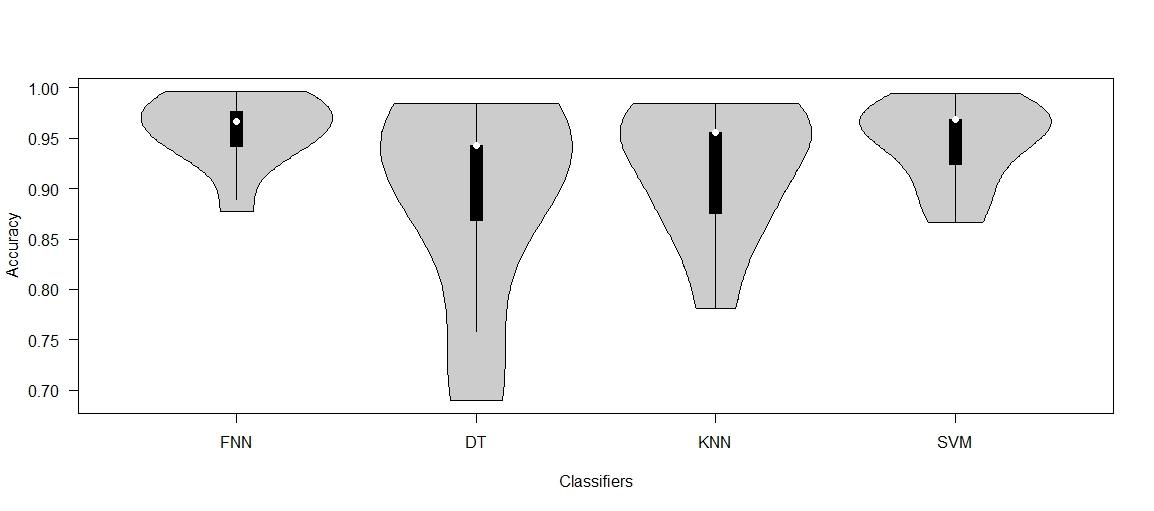
\includegraphics[width=14 cm]{Definitions/images/boxplot_overall_accuracy_4.jpeg}
	\caption{Comparison between classifiers in terms of accuracy}
	\label{fig:classification_comparison}
\end{figure}
 Figure \ref{fig:classification_comparison} shows how results of each classifier are spread out over 10 rounds. FNN followed by SVM show a range between 85\% through 99\% of accuracy over 10 trials while DT and KNN are showing more divergence over trials respectively between (75\%-98\%) and (78\%-98\%) of performances. Obviously, The median for accuracy of all classifiers are closely around 95\% whereas only for FNN's result, the 3rd quartile is located above the 98\%. The 3rd quartile for other classifiers are equal to their median. This is to say that this result is also promising to achieve a better performance for more number of trials.
A expected and confirmed by our results in RQ1, different classifiers perform differently. Hence, one question that we aim to answer is whether certain classifiers perform better than others. Therefore, in this research question we do an empirically compare the performance of different classifiers in HAR. We use four popular classifiers in HAR including SVM, KNN, FNN, and DT. It is important to mention that we evaluate the model using default configurations. We are not looking for optimal setup of each classifier \emad{so which configuration do we use? Default?}. \hosein{it is not different from what we said in the methodology/classification.}

Table~\ref{accuracy_classifier_featureset} summarizes the classification results for each classifier over all featuresets.  From analysing the behaviour of classifiers, it emerges that \textbf{FNN and SVM provide the best results on all featuresets, allowing to correctly recognize activities on average 89.04\% and 87.82\% of data points, respectively}. On the other hand, the other classifiers achieve an accuracy of 85.50\% and 82.83\% of accuracy for KNN and DT, respectively. Overall, the highest accuracy achieved by the FNN is 95.89\% for Histogram features \textit{set\_B}, while the worst accuracy is 74.02\% obtained by DT. In the majority of the cases, the classifiers follow same accuracy performance patterns over different featuresets, i.e., ST\_Set and HB\_Set perform best, followed by SS\_Set, PH\_Set and OI\_Set. 


\subsubsection{RQ3: How do different evaluation methods impact the reported HAR performance?}

K-fold is one of the most popular methods to evaluate the performance of a HAR model~\cite{wang2019survey}. However, in an empirical study, Jordao et al.~\cite{jordao2018human} showed that the result of k-fold cross validation can be biased when using sliding windows, a technique that is commonly used in HAR. Therefore, the focus of this research question is to asses models by two state-of-the-art evaluation methods namely, Leave-One-Subject-Out (LOSO) cross validation~\cite{liu2011multisensor} and Leave-One-Trial-Out (LOTO) Cross validation~\cite{sena2018multiscale,jordao2018human}. 

Table \ref{dataset_destribution} shows how the data is separated in each validation method based on number of activities and number of subjects. In K-fold, splitting the dataset is decided by researcher based on the size and distribution of dataset as well as type of classification problem\cite{jordao2018human}. However, in LOSO and LOTO it is up to number of participants and number of sets that they repeat same activities, respectively. In this experiment, for LOSO we used data of 5 activities coming from 4 subjects. For LOTO, we have employed the data of 7 activities from 4 subjects. It is important to mention that, in LOTO, finding a session of data from one subject including enough common exercises to be trained and test on is the main reason that does not let us to employ all recorded sessions of the dataset. Same limitation on finding data from one subject is applicable for LOSO.

\begin{table}[H]
	\caption{The distribution of activities, repetitions, and subjects among three evaluation methods as well as how the data set splits in each one. }
	\centering
	\begin{tabular}{p{4cm}p{2.2cm}p{2.2cm}p{2.2cm}p{2.2cm}}
		\toprule
		\textbf{Evaluation Method} & \textbf{\# Activities} & \textbf{\# Repeats}  & \textbf{\# Subjects}& \textbf{\# splits}\\
		\midrule
		K-Fold &  8 & 26 & 13 & 10 \\
		LOTO & 7 & 4& 6& 4  \\
		LOSO & 5 & 4 & 4& 4  \\
		\bottomrule
	\end{tabular}
	\label{dataset_destribution}
\end{table}
Figure~\ref{fig:evaluation_comparison} compares the performance of models using 10-fold cross validation (in blue), LOTO (in orange), and LOSO (in grey). As we can see from the Figure, for all featuresets and all classifiers, the evaluation technique impacts the reported performance. In fact, we see that in general, k-fold cross validation always provides better results than LOTO and LOSO. As mentioned earlier, due to the use of sliding windows in HAR, LOTO or LOSO are more realistic evaluation techniques and than k-fold cross validation. It can be seen that there is a significant distance between results of LOTO and LOSO (~10\%). This can be due to differently performing an exercise by different subjects in LOSO. However, in LOTO, since the model is trained by the data of at least one session of each subject it returns a better result. 

%For each classifier, results in the left columns have been obtained using 10-Fold evaluation, in middle columns using LOTO cross validation, and the right columns using LOSO cross validation. From the results, independent from featureset / classifier, it is obvious that the evaluating by LOTO or LOSO gives a lower performance (on average ~6\% and ~16\% respectively).
%Because of having an overlap between every consecutive data points due to using sliding window, a part of data which is used to generate a data point for train set will be used in data points for test set as well (96\% identical in this case). Therefore, We basically expect the performance achieved with k-fold to be higher than other methods because there is a significant correlation between train set and test set in this method. In other words, in K-fold, first, we generate data points from raw data (using sliding window), then, split them into test set and train set. However, in two other evaluation methods, training set and testing set are generated independently. So, the results are turned out from a less correlated test set thereby showing more realistic result, comparing with baseline. It can be seen that there is a significant distance between results of LOTO and LOSO (~10\%). This can be due to differently performing an exercise by different subjects in LOSO. However, in LOTO, since the model is trained by the data of at least one session of each subject it returns a better result. To compare classifiers, still FNN and SVM deliver the best result on all featuresets.

 
\begin{figure}[H]
	\centering
	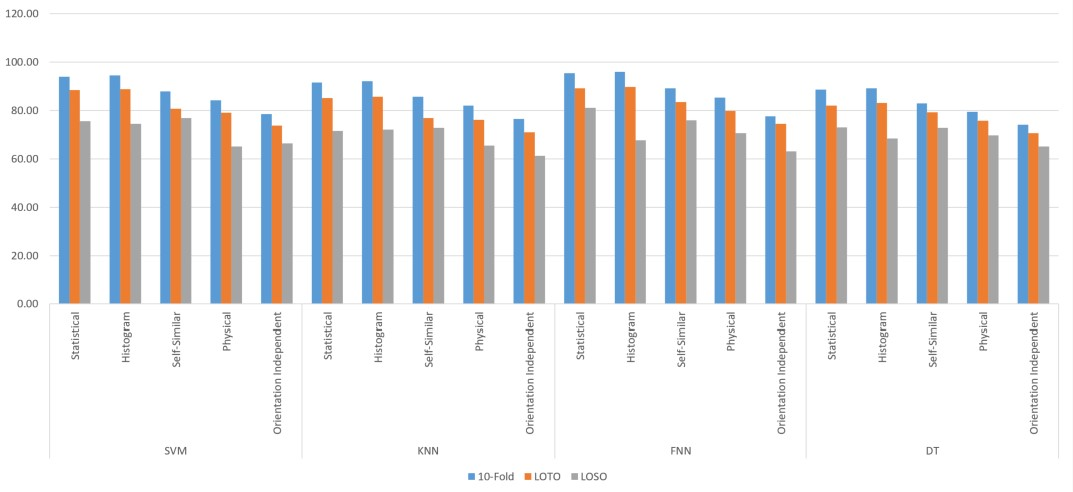
\includegraphics[width=14 cm]{Definitions/images/evaluation_comparison_2.jpg}
	\caption{Comparison between evaluation methods (10-Fold, LOTO, LOSO)}
	\label{fig:evaluation_comparison}
\end{figure} 

\begin{table}[H]
	\caption{Accuracy for each classifier and for all each feature-set using Leave-One-Trial-Out cross validation }
	\centering
	\begin{tabular}{p{3cm}p{2cm}p{2cm}p{2cm}p{2cm}p{2cm}}
		\toprule
		\textbf{Classifier} & \textbf{Set\_A} & \textbf{Set\_B} & \textbf{Set\_C} & \textbf{Set\_D} & \textbf{Set\_E} \\
		\midrule	
		SVM &  \cellcolor{gray!35}{76.73\%} & 73.11\% & \cellcolor{gray!35}{76.70}\% &69.19\% & 62.13\% \\
		KNN & 72.91\% & 75.58\% & 74.24\% &70.36\% & 61.74\% \\
		FNN & \cellcolor{gray!35}{77.07}\% & \cellcolor{gray!35}{79.87\%} &  \cellcolor{gray!35}{76.06\%} &\cellcolor{gray!35}{73.04\%} & 66.60\% \\
		DT & 69.48\% & 71.70\% & 72.58\% &71.18\% & 65.34\% \\
		\bottomrule
	\end{tabular}
	\label{Table:LOTO_results}
\end{table}

\begin{table}[H]
	\caption{Accuracy for each classifier and for all each feature-set using Leave-One-Subject-Out cross validation }
	\centering
	\begin{tabular}{p{3cm}p{2cm}p{2cm}p{2cm}p{2cm}p{2cm}}
		\toprule
		\textbf{Classifier} & \textbf{Set\_A} & \textbf{Set\_B} & \textbf{Set\_C} & \textbf{Set\_D} & \textbf{Set\_E} \\
		\midrule	
		SVM &  \cellcolor{gray!35}{68.83\%} & 69.11\% & \cellcolor{gray!35}{76.70}\% &69.19\% & 62.13\% \\
		KNN & 72.91\% & 75.58\% & 74.24\% &70.36\% & 61.74\% \\
		FNN & \cellcolor{gray!35}{77.07}\% & \cellcolor{gray!35}{79.87\%} & 76.06\% &\cellcolor{gray!35}{73.04\%} & 66.60\% \\
		DT & 69.48\% & 71.70\% &  \cellcolor{gray!35}{72.58\%} &71.18\% & 65.34\% \\
		\bottomrule
	\end{tabular}
	\label{Table:LOSO_results}
\end{table}

\emad{Are Tables 5 and 6 ever referenced to in the text?}\hosein{I wasn't sure to put them or remove them.}

\section{Discussion}
\subsection{Performance of FNN}
In this section we focus on investigating the FNN model on Histogram bins more in detail. 
Figure \ref{fig:fnn_hbins_confusion_matrix} shows the normalized confusion matrix for FNN model on \textit{set\_B}. One can see that activities such as Lat Pull Down and Bench Press (A1 and A2) are classified more accurately than activities such as Crunch Twist (A7) which is misclassified as Russian Twist (A8). In other words, it can be said that activities of a similar nature are more willing to get misclassified. Especially when the subject is not experienced enough on performing the exercise, recognizing the activity get harder. Addition to this the class A0 which stands for non-exercise activity is misclassified 1 percent as almost all other classes. This could be a result of variation in the distribution of data for all classes. This can also be illustrated in Figure \ref{fig:fnn_hbins_confusion_matrix} where the accuracy at first row is distributed across all the classes. Because of the uniform nature of data distribution among all classes, and because of a balanced nature, similar activities could be classified more accurately.\\
\begin{figure}[H]
	\centering
	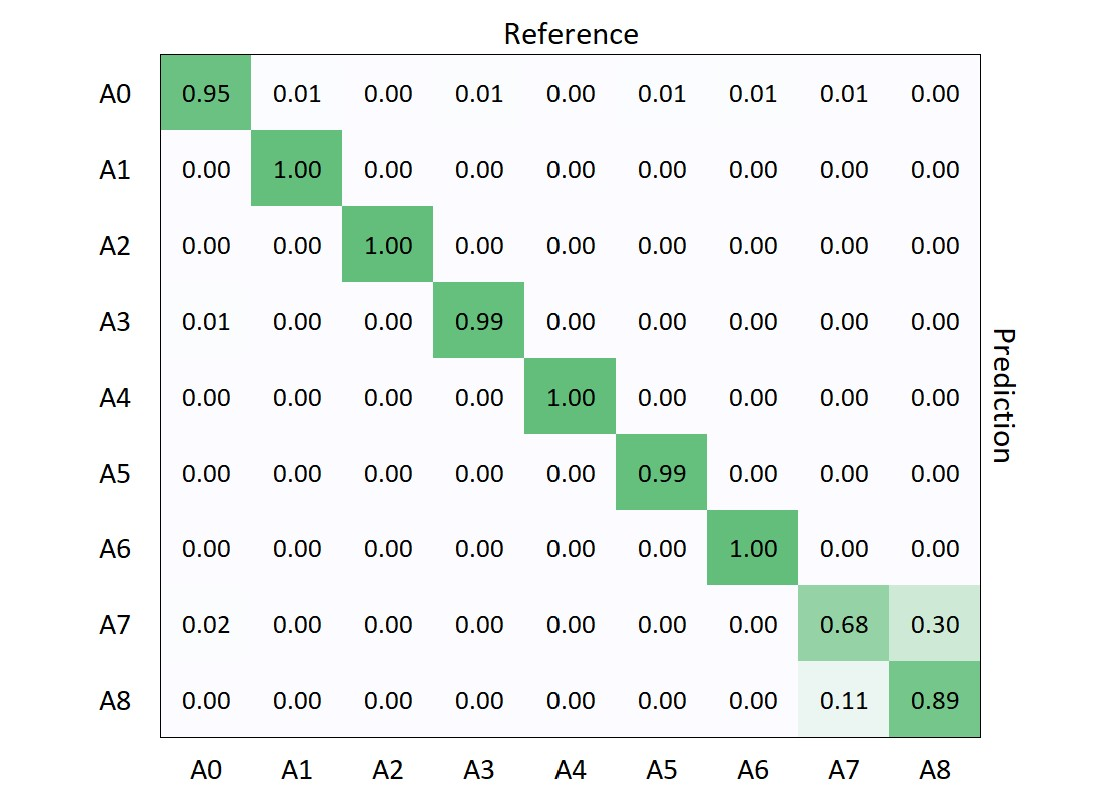
\includegraphics[width=7 cm]{Definitions/images/fnn_histogram_set.jpg}
	\caption{Normalized confusion matrix for FNN classifier using histogram dataset(set\_B). A0 in this table stands for non-exercise data points.}
	\label{fig:fnn_hbins_confusion_matrix}
\end{figure} 

\hosein{regarding We observe that when the standard activity recognition system is used with randomly oriented sensors (the random rotation case), the accuracy drops by 21.21\% on the average}
%\hosein{Since we already mention this aspect in RQ3, we may want to remove this subsection:\\
%\subsection{K-fold Evaluation result is biased?}
%As we argued earlier, each process has a drawback that might cause a negative impact on the methods. For instance, SNOW can produce biased results and the FNOW generates few samples. To face these problems, we propose the Leave-One-Trial-Out (LOTO) sample generation process.
%From the literature, the most popular method to evaluate a HAR model is K-fold cross-validation. In this method the data splits into k equal parts. The k-1 parts go for training and one part left for test. This process repeats for each k, separately. Main aim of this method is to keep the test and train part separate from each other and use all the samples in train and test. However, in case of using the conventional sliding window (with n\% overlap) for generating data-samples it is impossible for samples to be completely separated from each other. It is because of the overlap period which is common between each two windows in a sequence. In other words, as mentioned in \cite{jordao2018human}, the result is always biased because n\% of the data are identical between test and train part. To avoid this drawback, a ordinary evaluation method is Leave-One-Subject-Out (LOSO). Basically, this method resembles the k-fold cross-validation in which a fold is replaced by a subject. This method is secure against being biased since the data from each subject has no common area with other subjects. However, in order to have the performance in a satisfactory level, we have to increase the number of subjects, respectively. The Leave-One-Trial-Out (LOTO) cross-validation\cite{jordao2018human} is similar to LOSO, but use the data of a trial instead of a subject. Thus, we have ensured that the samples are basically separated and the performance does not depend on the number of subjects any more.
%\hosein{+ showing it in a example}
%}
%\subsection{Hand-Crafted Features VS Automated Features}

%The extraction of hand-crafted features are computationally lightweight and efficient to implement especially in ubiquitous devices. In addition, they are easy to understand due to the physical meanings of the features and finally, they work well for many HAR problems. However, choosing the right feature may be challenging based on the type of the problem underhand and also extracting the appropriate set of features depends on domain knowledge. \\
%In recent years, in parallel with the advancement of deep learning in many fields such as speech recognition and natural language processing, Deep Learning (DL) approaches have been explored in HAR. While most conventional methods use hand-crafted feature extraction, DL performs automatic high-level feature extraction thereby relieving the effort on designing features. In fact, instead of extracting feature manually, we train a neural network with raw input data from sensor. The strength of the automatically learned features by the deep networks is that the learning can be very deep, and the learning process does not rely on domain knowledge. In terms of performance, to the best of our knowledge, although there are researchs on both models, there is no comprehensive comparison to show a DL model how much better than a model on  a given hand-crafted features.\\
%In this section, we setup an experiment to compare the performance of a state-of-the-art Convolutional Neural Network (CNN) with the performance of the best model achieved in RQ3. 
%The input to the neural network consists of the reshaped sensor data from multiple sensors. Considering 5-second sliding window with 0.2 second shifting size (same setup as RQ1). Considering 50Hz sampling rate and three axes for each of the accelerometer and gyroscope sensors of two Neblinas, in total for one input window (channel), we have a matrix with three dimensions (5 * 50 * 12). This means that we stack the sensors on top of each other in a single channel. Table \ref{Table:CNN_network} shows the architecture of the network.

%Results achieved from this experiment has been shown in Figure \ref{cnn_result}.
%\begin{figure}[H]
%	\centering
%	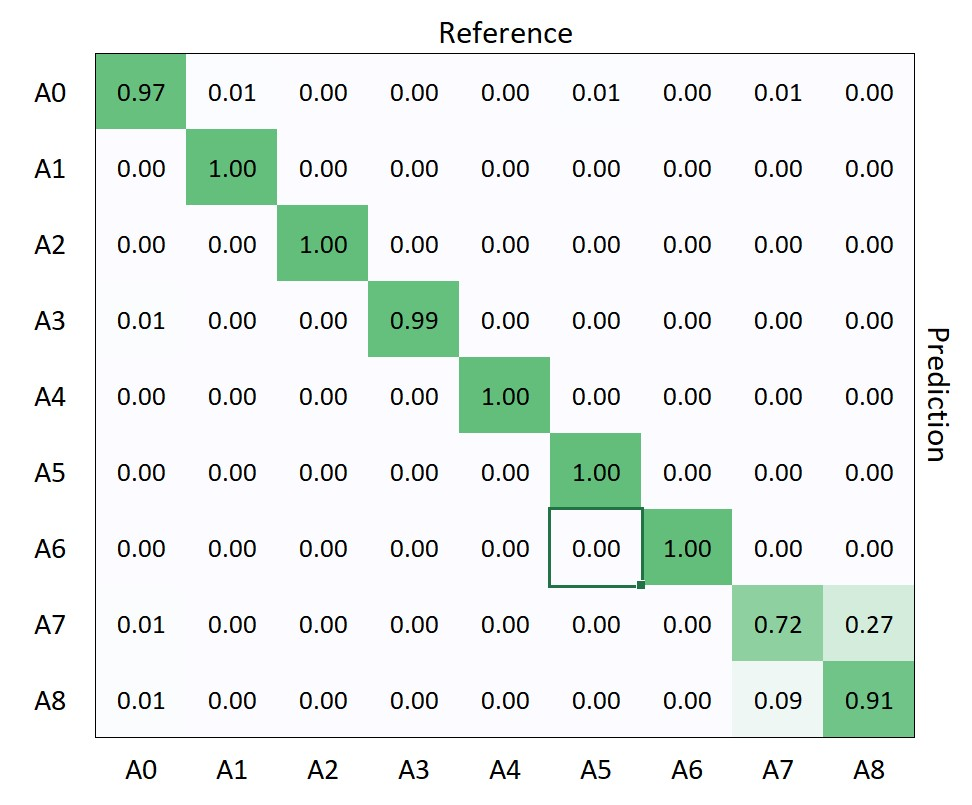
\includegraphics[width=7 cm]{Definitions/images/cnn_confusion.jpg}
%	\caption{Normalized confusion matrix for CNN classifier. A0 in this table stands for non-exercise data points.}
%	\label{cnn_result}
%\end{figure} 
%We evaluate the model using a 10-fold cross validation (same setup as RQ1). on average, the accuracy of the model in recognizing the activities is 96.11\% which is 0.22\% better than the best accuracy achieved by FNN model on histogram bins features. To investigate the performance of the model on  recognizing each activity, Figure \ref{cnn_results} shows the confusion matrix of the CNN model.

%\begin{table}[H]
%	\caption{Summary of the CNN model layers, output shape, and number of parameters }
%	\centering
%	\begin{tabular}{p{8cm}p{3cm}}
%		\toprule
%		\textbf{Layer} & \textbf{Value}  \\
%		\midrule	
%		Input shape &  250 * 12 * 1 \\
%		Convolutional filters CL1 &  100 \\
%		Kernel size CL1 &  (15, 3) \\
%		Strides CL1 &  (1, 3) \\
%		Convolutional filters CL2 &  25 \\
%		Kernel size CL2 &  (15, 18) \\
%		Strides CL2 &  (3, 1) \\
%		Convolutional filters CL3 &  75 \\
%		Kernel size CL3 &  (15, 18) \\
%		Strides CL3 &  (3, 1) \\
%		Convolutional filters CL4 &  75 \\
%		Kernel size CL4 &  (15, 18) \\
%		Strides CL4 &  (3, 1) \\
%		Convolutional filters CL5 &  25 \\
%		Kernel size CL5 &  (15, 18) \\
%		Strides CL5 & (3, 1)  \\
%		Activation function CL1, CL2, CL3, CL4, CL5 &  relu   \\
%		Dropout CL1, CL2, CL3, CL4, CL5 & 0.50 \\
%		DL1 neurons & 250  \\
%		DL2 neurons & 8 \\
%		Activation function DL2 &  softmax \\
%		
%		\bottomrule
%	\end{tabular}
%	\label{Table:CNN_network}
%\end{table}

%\hosein{we may want to mention: in most daily HAR tasks, those methods may heavily rely on heuristic handcrafted feature extraction, which is usually limited by human domain knowledge (Bengio, 2013) 
%Those work indicated that, when the HAR data is multi-dimensional and activities are more complex, more hidden layers can help the model train well since their representation capability is stronger (Bengio, 2013) }

\subsection{Learning Speed }
The last but not the least aspect worthy to mentioned is various converging speed of FNN between using different featuresets. As mentioned in RQ1, training an FNN on Histogram bins after 100 epochs delivers the best performance comparing with result of training at same number of epochs on other featuresets. In this section, we investigate velocity of FNN on reaching its best performance during first 100 epochs. Figure \ref{fig:fnn_learning_speed} shows the accuracy of FNN models using different featuresets. As we expect, after 100 epochs, the models on histogram bins, statistical features, self-similarity features have been reached a higher level of accuracy (all above 90\%) while the had been stable almost after first 20 epochs. On the other hand, the trend for both models on physical features and orientation independent are below 90\% while they have not been stable even at greater number of epochs (close to 100). This is to say that FNN can be trained faster when it is feed with histogram bins, statistical features, or self-similarity features rather two other featuresets. Interesting, for FNN on histogram features, the first time to touch the best accuracy is at the 5th epoch. This number for models on statistical features and self-similarity features happens after 14 epochs and 12 epochs respectively.

\begin{figure}[H]
	\centering
		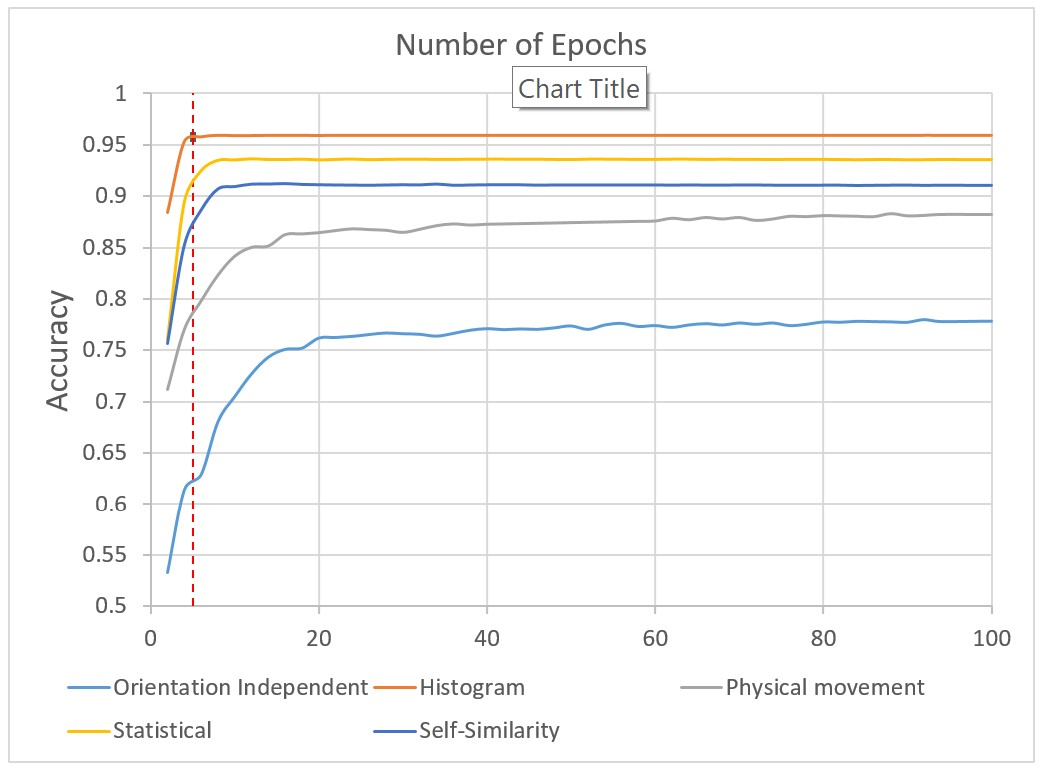
\includegraphics[width= 10cm]{Definitions/images/fnn_learning_speed.jpg}
		\caption{Accuracy of FNN during first 100 epochs using 5 featuresets}
		\label{fig:fnn_learning_speed}
\end{figure} 


%%%%%%%%%%%%%%%%%%%%%%%%%%%%%%%%%%%%%%%%%%
\section{Conclusions}

Human activity recognition is an important research topic
in pattern recognition and pervasive computing. In this paper, we have studied on the state-of-the-art models using hand-crafted features and traditional models. From RQ1 and RQ2, it turned out that FNN and histogram bins can deliver a superior performance rather other 19 pairs of classifiers and featuresets. It is also important to mention that the number of bins and width of each bin play important roles on extracting informative features. In RQ3, comparing leave-one-trial-out cross validation with two conventional evaluation methods (k-fold and LOSO), we saw that LOTO and LOSO provide a more realistic result rather K-Fold at the expense of declining the accuracy. Addition to this, we figured out, LOTO can address two issues which are not solved LOSO, including: 1) it is applicable on datasets with less number of subjects comparing with LOSO which requires more subjects. 2) it can suppress the impact of performing differently of an exercise by different subjects. 

%%%%%%%%%%%%%%%%%%%%%%%%%%%%%%%%%%%%%%%%%%
\vspace{6pt} 

%%%%%%%%%%%%%%%%%%%%%%%%%%%%%%%%%%%%%%%%%%
%% optional
%\supplementary{The following are available online at \linksupplementary{s1}, Figure S1: title, Table S1: title, Video S1: title.}

% Only for the journal Methods and Protocols:
% If you wish to submit a video article, please do so with any other supplementary material.
% \supplementary{The following are available at \linksupplementary{s1}, Figure S1: title, Table S1: title, Video S1: title. A supporting video article is available at doi: link.}

%%%%%%%%%%%%%%%%%%%%%%%%%%%%%%%%%%%%%%%%%%
\authorcontributions{For research articles with several authors, a short paragraph specifying their individual contributions must be provided. The following statements should be used ``conceptualization, X.X. and Y.Y.; methodology, X.X.; software, X.X.; validation, X.X., Y.Y. and Z.Z.; formal analysis, X.X.; investigation, X.X.; resources, X.X.; data curation, X.X.; writing--original draft preparation, X.X.; writing--review and editing, X.X.; visualization, X.X.; supervision, X.X.; project administration, X.X.; funding acquisition, Y.Y.'', please turn to the  \href{http://img.mdpi.org/data/contributor-role-instruction.pdf}{CRediT taxonomy} for the term explanation. Authorship must be limited to those who have contributed substantially to the work reported.}

%%%%%%%%%%%%%%%%%%%%%%%%%%%%%%%%%%%%%%%%%%
\funding{Please add: ``This research received no external funding'' or ``This research was funded by NAME OF FUNDER grant number XXX.'' and  and ``The APC was funded by XXX''. Check carefully that the details given are accurate and use the standard spelling of funding agency names at \url{https://search.crossref.org/funding}, any errors may affect your future funding.}

%%%%%%%%%%%%%%%%%%%%%%%%%%%%%%%%%%%%%%%%%%
\acknowledgments{In this section you can acknowledge any support given which is not covered by the author contribution or funding sections. This may include administrative and technical support, or donations in kind (e.g., materials used for experiments).}

%%%%%%%%%%%%%%%%%%%%%%%%%%%%%%%%%%%%%%%%%%
\conflictsofinterest{Declare conflicts of interest or state ``The authors declare no conflict of interest.'' Authors must identify and declare any personal circumstances or interest that may be perceived as inappropriately influencing the representation or interpretation of reported research results. Any role of the funders in the design of the study; in the collection, analyses or interpretation of data; in the writing of the manuscript, or in the decision to publish the results must be declared in this section. If there is no role, please state ``The funders had no role in the design of the study; in the collection, analyses, or interpretation of data; in the writing of the manuscript, or in the decision to publish the results''.} 

%%%%%%%%%%%%%%%%%%%%%%%%%%%%%%%%%%%%%%%%%%
%% optional
\abbreviations{The following abbreviations are used in this manuscript:\\
	
	\noindent 
	\begin{tabular}{@{}ll}
		MDPI & Multidisciplinary Digital Publishing Institute\\
		DOAJ & Directory of open access journals\\
		TLA & Three letter acronym\\
		LD & linear dichroism
\end{tabular}}

%%%%%%%%%%%%%%%%%%%%%%%%%%%%%%%%%%%%%%%%%%
%% optional
\appendixtitles{no} %Leave argument "no" if all appendix headings stay EMPTY (then no dot is printed after "Appendix A"). If the appendix sections contain a heading then change the argument to "yes".
\appendix
\section{}
\unskip
\subsection{}
The appendix is an optional section that can contain details and data supplemental to the main text. For example, explanations of experimental details that would disrupt the flow of the main text, but nonetheless remain crucial to understanding and reproducing the research shown; figures of replicates for experiments of which representative data is shown in the main text can be added here if brief, or as Supplementary data. Mathematical proofs of results not central to the paper can be added as an appendix.

\section{}
All appendix sections must be cited in the main text. In the appendixes, Figures, Tables, etc. should be labeled starting with `A', e.g., Figure A1, Figure A2, etc. 

%%%%%%%%%%%%%%%%%%%%%%%%%%%%%%%%%%%%%%%%%%
% Citations and References in Supplementary files are permitted provided that they also appear in the reference list here. 

%=====================================
% References, variant A: internal bibliography
%=====================================
\reftitle{References}
%\begin{thebibliography}{999}
%	% Reference 1
%	\bibitem[Author1(year)]{ref-journal}
%	Author1, T. The title of the cited article. {\em Journal Abbreviation} {\bf 2008}, {\em 10}, 142--149.
%	% Reference 2
%	\bibitem[Author2(year)]{ref-book}
%	Author2, L. The title of the cited contribution. In {\em The Book Title}; Editor1, F., Editor2, A., Eds.; Publishing House: City, Country, 2007; pp. 32--58.
%\end{thebibliography}

% The following MDPI journals use author-date citation: Arts, Econometrics, Economies, Genealogy, Humanities, IJFS, JRFM, Laws, Religions, Risks, Social Sciences. For those journals, please follow the formatting guidelines on http://www.mdpi.com/authors/references
% To cite two works by the same author: \citeauthor{ref-journal-1a} (\citeyear{ref-journal-1a}, \citeyear{ref-journal-1b}). This produces: Whittaker (1967, 1975)
% To cite two works by the same author with specific pages: \citeauthor{ref-journal-3a} (\citeyear{ref-journal-3a}, p. 328; \citeyear{ref-journal-3b}, p.475). This produces: Wong (1999, p. 328; 2000, p. 475)

%=====================================
% References, variant B: external bibliography
%=====================================
\externalbibliography{yes}
\bibliography{mybib}

%%%%%%%%%%%%%%%%%%%%%%%%%%%%%%%%%%%%%%%%%%
%% optional
\sampleavailability{Samples of the compounds ...... are available from the authors.}

%% for journal Sci
%\reviewreports{\\
%Reviewer 1 comments and authors’ response\\
%Reviewer 2 comments and authors’ response\\
%Reviewer 3 comments and authors’ response
%}

%%%%%%%%%%%%%%%%%%%%%%%%%%%%%%%%%%%%%%%%%%
\end{document}
